\documentclass{article}
\usepackage{booktabs,geometry,graphicx,amsmath}
\geometry{margin=1in}
\title{Covariate-shift tests on the stored DGP grid}
\author{}
\date{}
\begin{document}
\maketitle

This note aligns the MMD leave-one-coordinate scores with the project's own
batches. It is not the FSDS horse-race. Every draw stored in
\texttt{DGP\_whole\_outputs.npy} and \texttt{DGP\_whole\_outputs\_onesided.npy}
is tested once, after dropping duplicate configuration seeds. There are 377
draws, each with $n=1000$ reference rows, $n=1000$ new rows, and $d=10$
coordinates. The tests receive $X$ only.

The kernel statistics use $\exp(-\gamma\|x-y\|^2)$. The median bandwidth is
$1$ over the median pooled squared distance, computed on the whole pool and
held fixed across permutations. A second vanilla MMD uses $\gamma=1$, the
default argument of the uploaded \texttt{kernel\_MMD}. Both use the unbiased
U-statistic from Gretton et al.\ (2012), including division of the cross term
by $nm$. The uploaded function omits that divisor, which at this sample size
leaves a raw double sum in place of an average. LOCO subtracts one coordinate's
squared differences from the three distance matrices and is summarized by its
maximum and by the sum of its positive coordinates. The Xu statistic is the
uploaded adaptive sum-of-powers mean test. C2ST is the uploaded random forest
with depth $4$ and $B=19$ label permutations. Kernel tests use $49$
permutations. The Xu combination uses 199, because five powers each contribute
a zero rank and 49 permutations cannot push that combination under $0.05$.
A draw is counted as a rejection at $\alpha=0.05$.

Mean shift moves the first three coordinates. Covariance writes correlations
into two pairs. Mixture adds a point mass of size $2$ on the first three
coordinates with probability $\delta$. Support replaces the new batch with
a uniform on $[-\,(1+\delta),\,1+\delta]$. Concept drift is added only to $Y$.
Draws that share a covariate mechanism and a $\delta$, and differ only in the
concept drift, are replicates of the same $P(X)$.

On a mean shift, median-bandwidth MMD and both LOCO summaries reject every
stored draw, already at $\delta=0.25$. At that same point $\gamma=1$ rejects
$0.81$ and C2ST rejects $0.76$. Xu is a mean test once it has 199 permutations:
it follows the mean and mixture shifts and stays near the null on covariance
and support shifts.

The covariance shift is where the LOCO summaries pull apart from vanilla MMD.
At $\delta=0.50$ (21 draws) vanilla MMD rejects $0.57$, the maximum rejects
$0.76$ (5 draws only by the maximum, 1 only by MMD), and the positive sum
rejects every draw. At $\delta=0.25$ the order reverses: vanilla MMD rejects
$0.29$, the maximum $0.10$, and the positive sum $0.19$.

Support at $\delta=0.75$ is the bandwidth check. The new batch is uniform on
$[-1.75,1.75]$, whose variance matches the reference Gaussian. Median-bandwidth
MMD rejects $0.10$ of those draws and both LOCO summaries reject none.
$\gamma=1$ and C2ST reject all 21. On the other support values the median
kernel is back at rejection 1.

The 41 draws with no covariate shift, most of them concept drift only, give
rejection $0.049$ for median MMD, $0$ for the maximum, $0.024$ for the
positive sum, and $0.073$ for C2ST. A change in the regression does not move
a test that only sees $X$.

\begin{table}[p]
\centering
\caption{Rejection rate on the stored draws, pooled across concept-drift settings. Those settings change $Y$ only, so they are replicates of the same $P(X)$ shift. The null row is every draw with no covariate shift.}
\resizebox{\textwidth}{!}{%
\begin{tabular}{lllcccccc}
\toprule
shift & $\delta$ & $n$ & MMD & max LOCO & positive-sum LOCO & MMD $\gamma=1$ & Xu & C2ST \\
\midrule
covariance & 0.25 & 21 & 0.29 & 0.10 & 0.19 & 0.24 & 0.10 & 0.05 \\
covariance & 0.50 & 21 & 0.57 & 0.76 & 1.00 & 0.52 & 0.05 & 0.14 \\
covariance & 0.75 & 21 & 1.00 & 1.00 & 1.00 & 1.00 & 0.00 & 0.81 \\
covariance & 1.00 & 21 & 1.00 & 1.00 & 1.00 & 1.00 & 0.05 & 1.00 \\
mean & 0.25 & 21 & 1.00 & 1.00 & 1.00 & 0.81 & 1.00 & 0.76 \\
mean & 0.50 & 21 & 1.00 & 1.00 & 1.00 & 1.00 & 1.00 & 1.00 \\
mean & 0.75 & 21 & 1.00 & 1.00 & 1.00 & 1.00 & 1.00 & 1.00 \\
mean & 1.00 & 21 & 1.00 & 1.00 & 1.00 & 1.00 & 1.00 & 1.00 \\
mixture & 0.25 & 21 & 1.00 & 1.00 & 1.00 & 0.95 & 1.00 & 0.90 \\
mixture & 0.50 & 21 & 1.00 & 1.00 & 1.00 & 1.00 & 1.00 & 1.00 \\
mixture & 0.75 & 21 & 1.00 & 1.00 & 1.00 & 1.00 & 1.00 & 1.00 \\
mixture & 1.00 & 21 & 1.00 & 1.00 & 1.00 & 1.00 & 1.00 & 1.00 \\
none & 0.00 & 41 & 0.05 & 0.00 & 0.02 & 0.02 & 0.02 & 0.07 \\
support & 0.25 & 21 & 1.00 & 1.00 & 1.00 & 1.00 & 0.00 & 1.00 \\
support & 0.50 & 21 & 1.00 & 1.00 & 1.00 & 1.00 & 0.10 & 1.00 \\
support & 0.75 & 21 & 0.10 & 0.00 & 0.00 & 1.00 & 0.00 & 1.00 \\
support & 1.00 & 21 & 1.00 & 1.00 & 1.00 & 1.00 & 0.00 & 1.00 \\
\bottomrule
\end{tabular}}
\end{table}
\clearpage
\begin{table}[p]
\centering
\caption{Same tests, averaged inside each DGP label. \texttt{concept\_only} keeps $P(X)$ fixed and moves the regression.}
\resizebox{\textwidth}{!}{%
\begin{tabular}{lccccccc}
\toprule
label & $n$ & MMD & max LOCO & positive-sum LOCO & MMD $\gamma=1$ & Xu & C2ST \\
\midrule
concept\_only & 38 & 0.05 & 0.00 & 0.03 & 0.03 & 0.03 & 0.08 \\
covariate\_only & 32 & 0.91 & 0.88 & 0.91 & 0.94 & 0.50 & 0.88 \\
mixed & 304 & 0.87 & 0.87 & 0.88 & 0.90 & 0.52 & 0.85 \\
no\_shift & 3 & 0.00 & 0.00 & 0.00 & 0.00 & 0.00 & 0.00 \\
\bottomrule
\end{tabular}}
\end{table}
\clearpage


\begin{figure}[p]
\centering
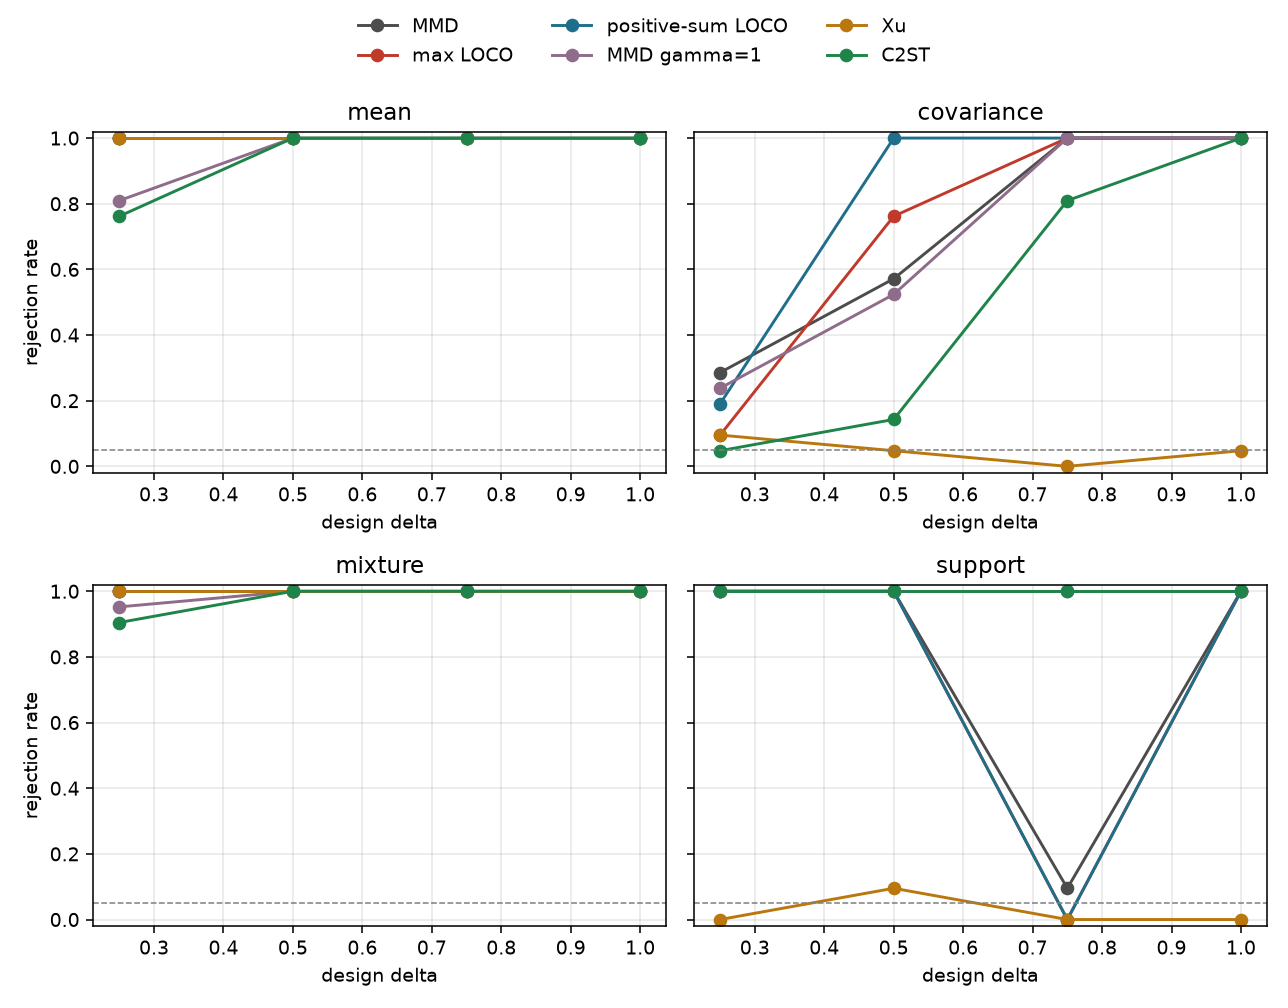
\includegraphics[width=\textwidth]{power.png}
\caption{Rejection rate against the design delta. Each panel is one covariate
mechanism. Concept-drift companions of the same mechanism are pooled.
The dashed line is $0.05$.}
\end{figure}
\end{document}
